% ============================================================
% ABOUT THE AUTHOR
% front_matter/about_author.tex
% ============================================================

\chapter*{About the Author}
\addcontentsline{toc}{chapter}{About the Author}
\markboth{About the Author}{About the Author}

\vspace{0.3cm}
\noindent
\begin{minipage}[t]{0.26\textwidth}
  \vspace{0pt}
  \centering
  {\setlength{\fboxsep}{2pt}\setlength{\fboxrule}{0.4pt}%
  \fbox{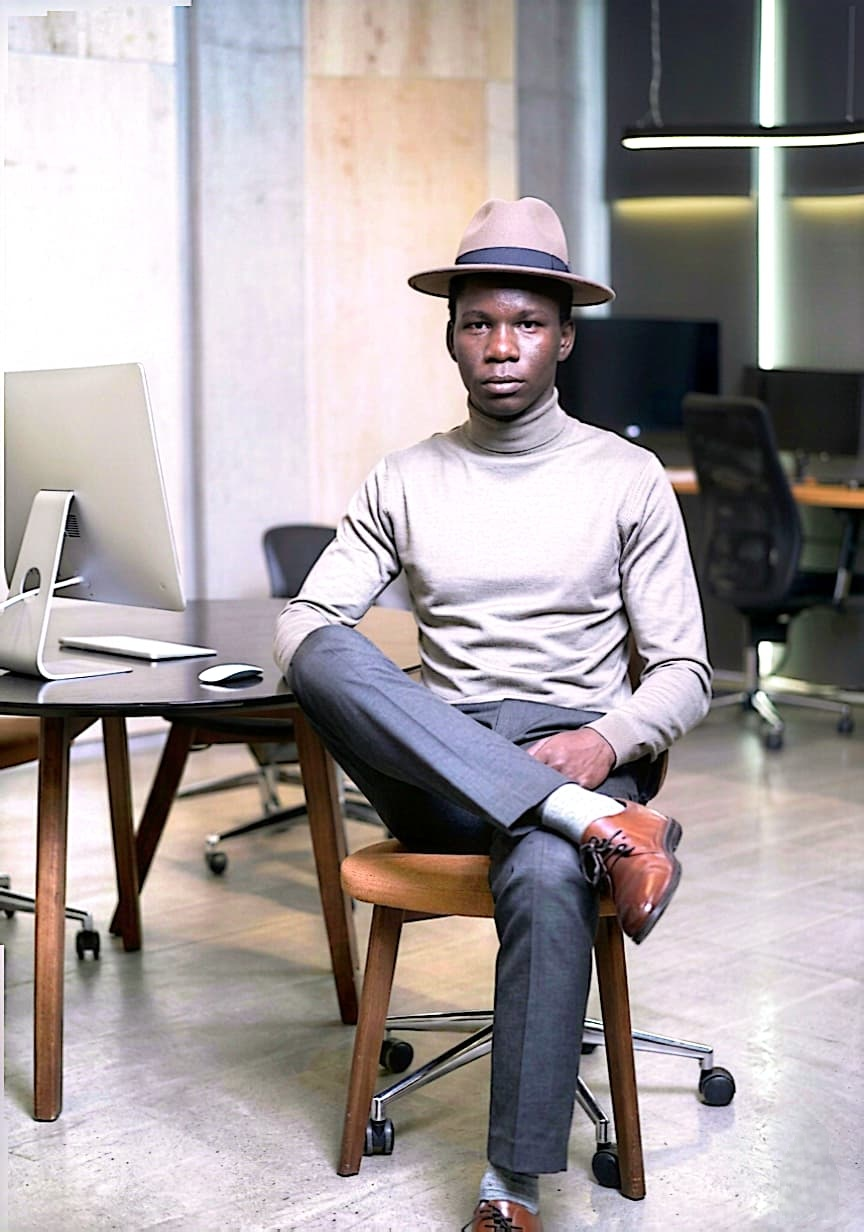
\includegraphics[width=3cm,height=4.2cm,keepaspectratio]{author_photo.png}}}
\end{minipage}%
\hfill
\begin{minipage}[t]{0.70\textwidth}
  \vspace{0pt}
  {\large\bfseries Korede Samuel Omotosho}\enspace{\normalsize(\textbf{Falcon})}\\[0.2cm]
  {\small\itshape Educator\enspace·\enspace Developer\enspace·\enspace Entrepreneur}\\[0.25cm]
  \rule{\linewidth}{0.4pt}\\[0.25cm]
  \textbf{Korede Samuel Omotosho}, widely known as \textbf{Falcon},
  is an 18-year-old Nigerian educator, developer, and entrepreneur
  whose work sits at the intersection of technology and education.
  He is the founder of \textbf{Aurikrex Learning Systems}, an
  education technology platform built to close the gap between
  how Nigerian students are taught and how they actually learn.
\end{minipage}

\vspace{0.35cm}

\noindent Falcon began teaching Physics, Mathematics, Further Mathematics, Chemistry, and Biology at a lesson center in Lagos, while simultaneously developing digital tools for students preparing for UTME and university entrance exams. His approach is grounded in a clear belief: any student—regardless of background or past performance—can achieve deep understanding in science when concepts are explained with clarity, honesty, and from first principles. Over time, he has taught across multiple centers, impacting more than 500 UTME and SSCE students.

\smallskip

\noindent He is the author of \textit{The UTME Physics Blueprint},
\textit{The UTME Chemistry Blueprint}, and
\textit{The UTME Biology Blueprint} --- a series of
high-efficiency revision guides used by UTME candidates
across Nigeria. \textit{The Physics Codex} is his first
full-length textbook, and the first volume in
\textit{The Aurikrex Codex Series}.

\smallskip

\noindent Beyond teaching, Falcon develops educational software including
SyncGrade, a CGPA calculator for Nigerian tertiary students,
and several digital learning tools designed specifically for
the Nigerian curriculum. His broader vision through Aurikrex
is to build a complete learning infrastructure for African
students --- one that does not merely prepare them for
examinations, but equips them to think, understand, and
create.

\smallskip

\noindent He lives and works in Lagos, Nigeria.

\vspace{0.4cm}
\begin{center}
\rule{0.45\linewidth}{0.4pt}\\[0.3cm]
{\small\itshape To connect with the author or learn more about Aurikrex Learning Systems:}\\[0.3cm]
\begin{tabular}{rl}
  \textit{Email:}    & \href{mailto:aurikrexacademy@gmail.com}{aurikrexacademy@gmail.com}\\[0.15cm]
  \textit{WhatsApp:} & \href{https://wa.me/2349113683395}{+2349113683395}\\
\end{tabular}
\end{center}
